\documentclass{beamer}
\usetheme{metropolis}
\usepackage{graphicx}
\usepackage{subfig}
\usepackage{tcolorbox}
\title{Calculus-Based Physics-2: Electricity, Magnetism, and Thermodynamics (PHYS180-02): Review}
\author{Jordan Hanson}
\institute{Whittier College Department of Physics and Astronomy}

\begin{document}
\maketitle

\section{Review}

\begin{frame}{Summary}
\begin{enumerate}
\item Chapter 5 - Electric charges and fields
\item Chapter 6 - Gauss' Law
\item Chapter 7 - Electric Potential
\item Chapter 8 - Capacitance
\item Chapter 9 - Current and Resistance
\item Chapter 10 - DC Circuits
\item Chapter 11 - Magnetic Forces and Fields
\item Chapter 12 - Sources of Magnetic Fields
\item Chapter 13 - Electromagnetic Induction
\item Chapter 14 - Inductance
\item Chapter 16 - Electromagnetic waves
\end{enumerate}
\end{frame}

\begin{frame}{Review}
\begin{columns}[T]
\begin{column}{0.5\textwidth}
\small
Two charges Q of mass 5.0 g, are attached to 50 cm strings, which are in turn tied to the same point, as shown.  The threads hang at 5.0 deg to the vertical, as shown below. What is the magnitude of Q? What are the signs of the two charges? \\ \vspace{0.5cm}
\textbf{Placing the charges in an upward pointing E-field would}
\begin{itemize}
\item A: Increase the angle slightly
\item B: Decrease the angle slightly
\item C: Not change the angle
\item D: Increase the angle to the max of 90 deg
\end{itemize}
\end{column}
\begin{column}{0.5\textwidth}
\begin{figure}
\centering
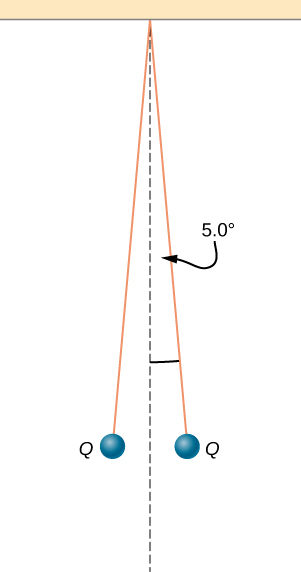
\includegraphics[width=0.5\textwidth]{ex1.jpeg}
\caption{\label{fig:ex1}}
\end{figure}
\end{column}
\end{columns}
\end{frame}

\begin{frame}{Review}
\begin{columns}[T]
\begin{column}{0.4\textwidth}
\small
Suppose the density of the oil droplets in the Millikan oil-drop experiment is 885 kg/m$^3$.  If the radii of the drops is observed to be 1 $\mu$m, what is the mass of the drops? \\ \vspace{0.5cm}
What is the weight of the drops in Newtons? \\
\vspace{0.5cm}
Suppose an E-field of 4545 N/C is required to hold the drops motionless.  How many electrons are on the drops, on average?
\end{column}
\begin{column}{0.6\textwidth}
\begin{figure}
\centering
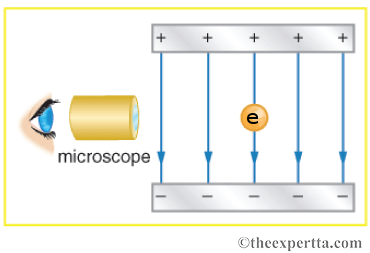
\includegraphics[width=0.5\textwidth]{ex2.png}
\caption{\label{fig:ex2}}
\end{figure}
\small 
If the field were increased in magnitude, the charges would:
\begin{itemize}
\item A: accelerate upwards
\item B: accelerate downwards
\item C: move down at constant v
\item D: move up at constant v
\end{itemize}
\end{column}
\end{columns}
\end{frame}

\begin{frame}{Review}
\begin{columns}[T]
\begin{column}{0.4\textwidth}
\small
Charge is distributed uniformly with a density $\rho$ throughout an infinitely long cylindrical volume of radius R. Show that the field of this charge distribution is directed radially with respect to the cylinder and that
\begin{align}
E &= \frac{\rho r}{2\epsilon_0}, ~ r\leq R\\
E &= \frac{\rho R^2}{2\epsilon_0 r}, ~ r>R
\end{align}
\end{column}
\begin{column}{0.6\textwidth}
\begin{figure}
\centering
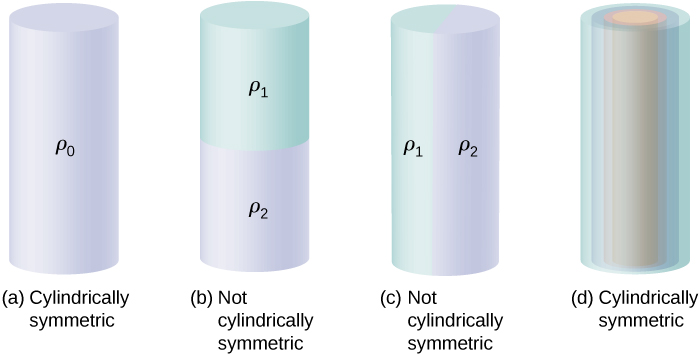
\includegraphics[width=0.95\textwidth]{cyl.jpeg}
\caption{\label{fig:cyl} Gauss' Law involves an understanding of symmetry.}
\end{figure}
\end{column}
\end{columns}
\end{frame}

\begin{frame}{Review}
\begin{columns}[T]
\begin{column}{0.5\textwidth}
\small
Suppose the capacitances $C_1$, $C_2$, and $C_3$ are all 5 $\mu$F.  What is the total capacitance? \\ \vspace{0.5cm}
Suppose $C_1 = C_2 = 5 \mu$F, but $C_3 = 100 \mu$F.  What is the total capacitance? \\ \vspace{0.5cm}
Suppose a 1 $\mu$F capacitor is connected in series with a $1$ k$\Omega$ resistor.  What is the RC time? \\ \vspace{0.5cm}
When will the capacitor in the RC circuit reach 90\% of the votlage of the charging battery?
\end{column}
\begin{column}{0.5\textwidth}
\begin{figure}
\centering
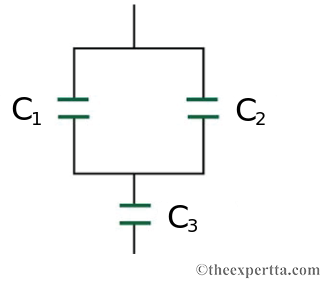
\includegraphics[width=0.95\textwidth]{ex3.png}
\caption{\label{fig:ex3}}
\end{figure}
\end{column}
\end{columns}
\end{frame}

\begin{frame}{Review}
\begin{columns}[T]
\begin{column}{0.5\textwidth}
\small
What equation do you get when you apply the loop rule to the loop abcdefgha, in terms of the variables in the figure? \\ \vspace{0.5cm}
If the current through the top branch is $I_2$ = 0.52 A, what is the current through the bottom, $I_3$, in amps? 
\end{column}
\begin{column}{0.5\textwidth}
\begin{figure}
\centering
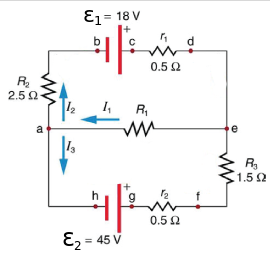
\includegraphics[width=0.95\textwidth]{ex4.png}
\caption{\label{fig:ex4}}
\end{figure}
\end{column}
\end{columns}
\end{frame}

\begin{frame}{Review}
\begin{columns}[T]
\begin{column}{0.65\textwidth}
\small
What is the value of the B-field a distance of 1 cm from a 10A current? (Recall Amp\`{e}re's Law). \\ \vspace{0.5cm}
If the current is cut in half, but the distance is doubled, what is the new B-field? \\ \vspace{0.5cm}
If two currents flowing in the same direction are placed near each other, they:
\begin{itemize}
\item A: repel each other always
\item B: attract each other always
\item C: repel each other if one changes
\item D: attract each other if one changes
\end{itemize}
\end{column}
\begin{column}{0.35\textwidth}
\begin{figure}
\centering
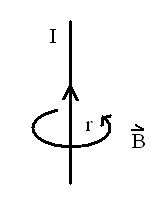
\includegraphics[width=0.95\textwidth]{ex5.png}
\caption{\label{fig:ex5}}
\end{figure}
\end{column}
\end{columns}
\end{frame}

\begin{frame}{Review}
\begin{columns}[T]
\begin{column}{0.65\textwidth}
\small
If the total number of turns in the loop is 500, and the frequency is 1000 Hz, what is the peak emf in the 0.03 T B-field? \\ \vspace{0.5cm}
Doubling the frequency, $f$, will
\begin{itemize}
\item A: Make the graph at bottom right oscillate more rapidly, but not raise the amplitude.
\item B: Raise the amplitude of the graph at bottom right.
\item C: Lower the amplitude of the graph at bottom right.
\item D: Both raise the amplitude of the graph at bottom right, and make it oscillate more rapidly.
\end{itemize}
\end{column}
\begin{column}{0.35\textwidth}
\begin{figure}
\centering
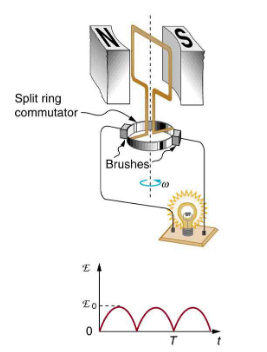
\includegraphics[width=0.95\textwidth]{ex6.png}
\caption{\label{fig:ex6}}
\end{figure}
\end{column}
\end{columns}
\end{frame}

\begin{frame}{Review}
\begin{columns}[T]
\begin{column}{0.45\textwidth}
\small
DC circuits:
\begin{equation}
P = i V
\end{equation}
In the problem at right, would the total current change if the devices were connected in series?
\begin{itemize}
\item A: Yes, it would increase
\item B: Yes, it would decrease
\item C: No change in total current
\item D: It would drop to zero
\end{itemize}
\end{column}
\begin{column}{0.65\textwidth}
An 1800-W toaster, a 1400-W electric frying pan, and a 75-W lamp are plugged into the same outlet in a 15-A, 120-V circuit. (The three devices are in parallel when plugged into the same socket.). (a) What current is drawn by each device? (b) Will this combination blow the 15-A fuse?
\end{column}
\end{columns}
\end{frame}

\section{Conclusion}

\begin{frame}{Summary}
\begin{enumerate}
\item Chapter 5 - Electric charges and fields
\item Chapter 6 - Gauss' Law
\item Chapter 7 - Electric Potential
\item Chapter 8 - Capacitance
\item Chapter 9 - Current and Resistance
\item Chapter 10 - DC Circuits
\item Chapter 11 - Magnetic Forces and Fields
\item Chapter 12 - Sources of Magnetic Fields
\item Chapter 13 - Electromagnetic Induction
\item Chapter 14 - Inductance
\item Chapter 16 - Electromagnetic waves
\end{enumerate}
\end{frame}

\end{document}
